% =============================================================================
% CPB-STIJL BEAMER TEMPLATE — Centraal Planbureau
% In LaTeX nagemaakt door Joep Tijm, Aisha Schmidt en ChatGPT
%
% Slide-types:
%   \cpbtitelframe              — Titelslide
%   \cpbinhoudframe{bullets}    — Inhoudslide
%   \begin{frame}{Titel}        — Contentslide
%   \cpbsection{Titel}{Sub}    	— Sectionslide
%   \cpbeindframe               — Eindslide
%
% Titelafbeelding (optioneel):
%   \cpbtitelafbeelding{pad.jpg}  — eigen afbeelding op linkerhelft titelslide
%   Zonder aanroep: Numbersbackground als placeholder
%
% Benodigd: rijkslogo.png, numbersbackground.png
% =============================================================================

\documentclass[aspectratio=169,11pt,handout,xcolor=dvipsnames]{beamer}

\usepackage[utf8]{inputenc}
\usepackage[T1]{fontenc}
\usepackage{cpb-beamer} % CPB colours, fonts, layouts and custom commands
\usepackage[dutch,english]{babel}  % Gebruik [english, dutch]{babel} voor nederlandse datumnotatie
\usepackage{booktabs}
\usepackage{colortbl}
\usepackage{array}
\newcommand{\mypos}[2]{\tikz[remember picture]{\node[inner sep=0pt, anchor=base](#2){#1};}}
\newcommand{\myund}{}
\usepackage{pgfplots}
\pgfplotsset{compat=1.18}
\usepackage{adjustbox}  % voor clippen van achtergrondafbeelding
\usepackage{setspace}
\usepackage{soul}
\usepackage{natbib} % voor using bibliographystyle amcg
\usepackage{bm}
\usepackage{amsmath,amsfonts,eqnarray}
\usepackage{amssymb,dsfont,bbold}
\usepackage{changepage}
\usepackage{nicefrac}
\usepackage{multirow}
\usepackage{subcaption}


\title[Short title]{Layout presentations CPB}
\author{A. Schmidt based on J. Tijm's template}
\disclaimer{Disclaimer}
\date{\today}
\cpbfooter{J. Tijm, A. Schmidt}
\cpbtitelafbeelding{Images/cover_bg.png} % Titel figuur

\begin{document}
\cpbtitelframe

% ==================
% ----  Teaser
% ==================


\begin{frame}{}
\vspace{1cm}
\begin{centering}
    \begin{block}{\centering Task}
        \centering{A block}
    \end{block}
\end{centering}
\pause
\vspace{1cm}
\begin{itemize}
    \item A list:
    \begin{itemize}
        \item Bullet 1
        \pause
        \item Bullet 2
    \end{itemize}
\end{itemize}
\end{frame}

% ==================
% ---- Agenda 
% ==================


\cpbinhoudframe{%
  \begin{itemize}
    \item A list:
    \begin{itemize}
        \item Bullet 1
        \pause
        \item Bullet 2
    \end{itemize}
\end{itemize}
}

% ==================
% ----  Section slide
% ==================

\cpbsectie{Section}{}

% ==================
% ---- Slide with Figure
% ==================

\begin{frame}{A title in the frame}
  \begin{itemize}
        \item References can be used using the references.bib file.
        \begin{itemize}
            \item You can cite \cite{lundberg2017} or \citep{lundberg2017}
        \end{itemize}
    \item We recommend adding the Figures in the Figures folder (you can also add subfolders if needed). 
    \begin{itemize}
        \item Reference by using Figure \ref{fig:example_figure}
        \item If the figures and tables order change, the numbers are automatically updated.
    \end{itemize}
\end{itemize}

\begin{figure}[H]
      \centering
      \vspace{-0.5cm}
      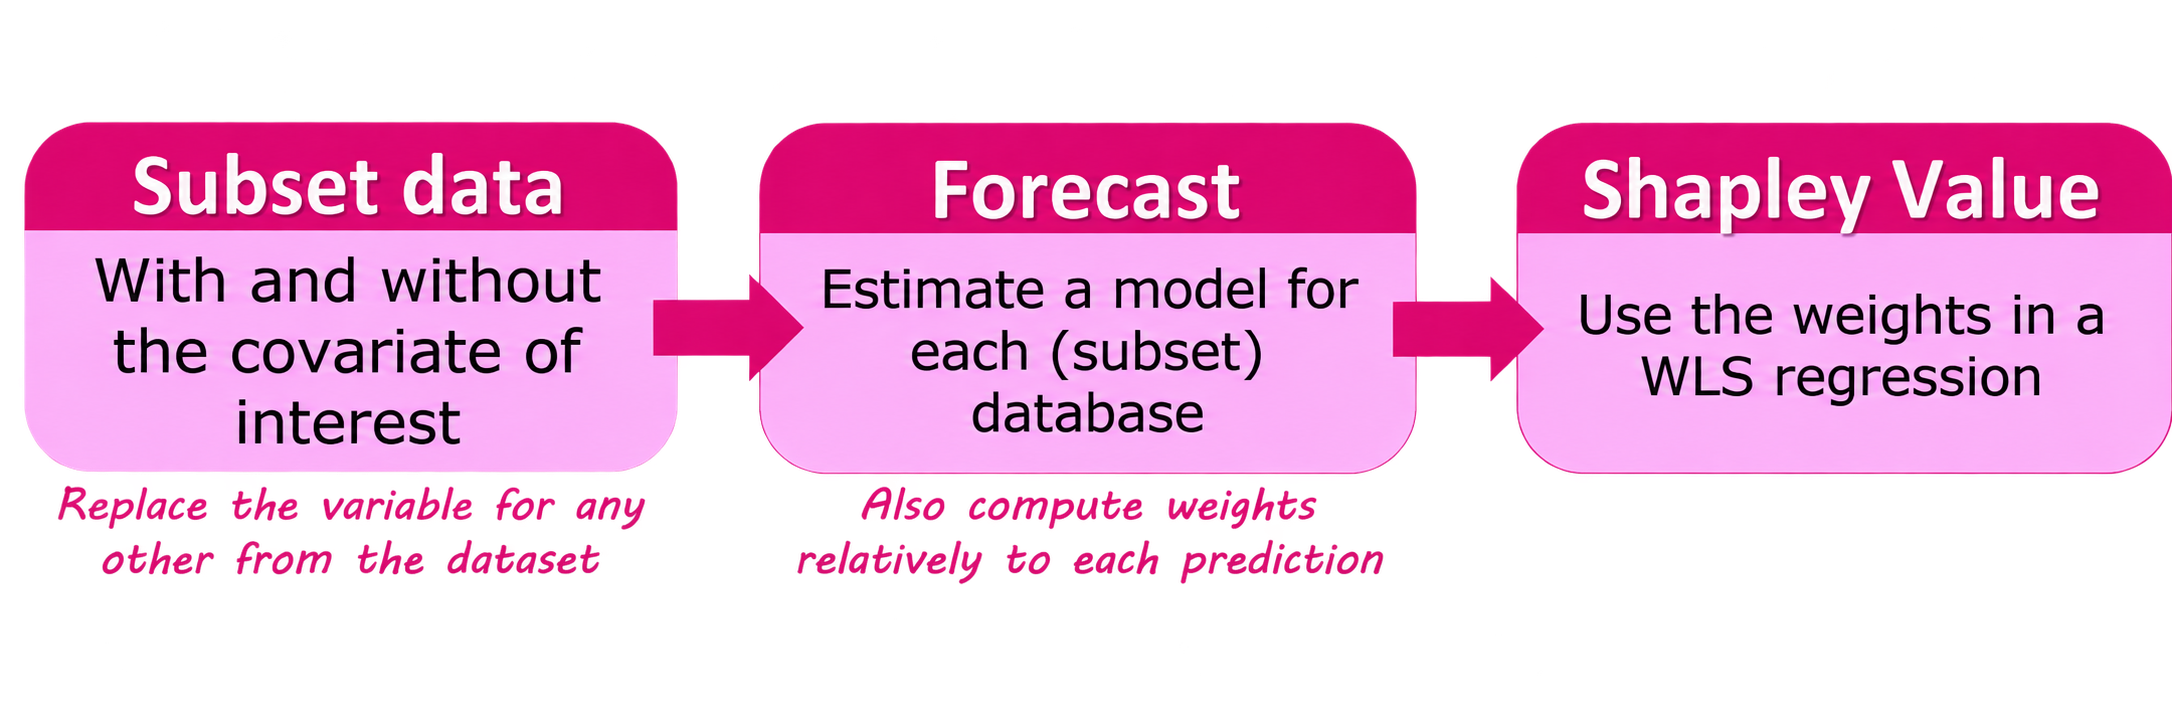
\includegraphics[scale=0.12]{Figures/SHAP2.png}
      \vspace{-0.5cm}
      \caption{\scriptsize{Example of a Figure}}
      \label{fig:example_figure}
\end{figure}
\end{frame}

% ==================
% ---- Slide with diagram
% ==================

\begin{frame}{Custom LaTeX diagrams}
\vspace{1cm}

  % Maximum 4 boxes
  \begin{figure}
    \centering
    \resizebox{0.6\linewidth}{!}{%
    \cpbdiagram{magenta}{4}{%
      \cpbdiagramitem
        {Box 1}
        {Text 1}
        {Caption 1}
      \cpbdiagramitem
        {Box 2}
        {Text 2}
        {Caption 2}
      \cpbdiagramitem
        {Box 3}
        {Text 3}
        {}
      \cpbdiagramitem
        {Box 4}
        {Text 4}
        {Caption 4}        
    }}
    \caption{Example of diagram made directly from the template}
    \label{fig:example_diagram_magenta}
  \end{figure}

  \begin{figure}
    \centering
    \resizebox{0.6\linewidth}{!}{%
    \cpbdiagram{blue}{3}{%
      \cpbdiagramitem
        {Box 1}
        {Text 1}
        {Caption 1}
      \cpbdiagramitem
        {Box 2}
        {Text 2}
        {Caption 2}
      \cpbdiagramitem
        {Box 3}
        {Text 3}
        {}      
    }}
    \caption{Example of a blue diagram made directly from the template}
    \label{fig:example_diagram_magenta}
  \end{figure}

  
\end{frame}


% ==================
% ---- Slide with table
% ==================


\begin{frame}[fragile]{Slide with table}

\scriptsize
\begin{itemize}
    \item You can add tables by creating a new file and adding it to the Tables folder
    \item You can also make reference to the objects by using Table \ref{tab:example_table}. This can be done with \verb|Table \ref{tab:example_table}|
\end{itemize}
\pause
\vspace{-0.5cm}
\begin{table}[!ht]
\begin{scriptsize}
\centering
\caption{Table example}
\scriptsize
\arrayrulecolor{cpbMagenta}
\begin{tabular}{clcccc}
\toprule
\multicolumn{2}{c}{ } & \multicolumn{2}{c}{In sample} & \multicolumn{2}{c}{Test} \\
\cmidrule(l{3pt}r{3pt}){3-4} \cmidrule(l{3pt}r{3pt}){5-6}
Horizon & Model & 10 vars & 15 vars & 10 vars & 15 vars\\
\midrule
 & Elastic net & 1.35 & 1.23 & 3.81 & 3.32\\

 & Lasso & 1.41 & 1.27 & 2.27 & 2.66\\

\multirow{-3}{*}{\centering\arraybackslash 1} & Random forest & 1.00 & 0.94 & 2.91 & 3.27\\
\cmidrule{1-6}
 & Elastic net & 7.24 & 6.72 & 7.46 & 4.49\\

 & Lasso & 7.56 & 5.70 & 8.77 & 2.94\\

\multirow{-3}{*}{\centering\arraybackslash 6} & Random forest & 2.31 & 2.14 & 17.11 & 17.62\\
\bottomrule
\end{tabular}
\label{tab:example_table}
\end{scriptsize}
\end{table}
\vspace{0.5em}
\raggedright
\scriptsize
\textbf{Note:} You can also add a footnote to add information about your figure or table.

\end{frame}

% ==================
% ---- Second section
% ==================

% Time series graphs

\cpbsectie{Another section}{Subtext}

%---

\begin{frame}[plain, fragile]
\label{slide:label_to_frame}
    \begin{itemize}
        \item You can have a slide without any decoration by using \verb|\begin{frame}[plain]|when starting your new frame
        \item You can also have navigation buttons by using \verb|\cpbbutton{appendix:01}{Go to Appendix}{inline}| \cpbbutton{appendix:01}{Go to Appendix}{inline}
        \item The position options are \verb|inline, bottom left, bottom right|
    \end{itemize}
\end{frame}



% ==================
% ---- End
% ==================

\begin{frame}
\begin{block}{What has been done $\ldots$}
    \begin{itemize}
        \item A Beamer template that follows CPB style
    \end{itemize}
\end{block}
\pause
\begin{block}{What else? $\ldots$}
    \begin{itemize}
        \item You can develop this template further as you want
    \end{itemize}
\end{block}   
\end{frame}

% ==================
% ---- End frame 
% ==================

\cpbeindframe

% ==================
% ---- Appendix 
% ==================


\begin{frame}[noframenumbering]{Appendix slide}
\label{appendix:01}
 \begin{itemize}
     \item You can use these Appendix slides to add extra information
     \item Navigation can be done with buttons that link to other slides
        \begin{itemize}
            \item For that, you need to add labels to your slides such that the buttons have the right references
        \end{itemize}
 \end{itemize}
     \cpbbutton{slide:label_to_frame}{Back}{bottom right}
\end{frame}


% ==================
% ---- References 
% ==================

\begin{frame}[noframenumbering,allowframebreaks=0.75]{Bibliography}
        \bibliographystyle{agsm}
        \bibliography{references}
\end{frame}



\end{document}
